\chapter{Sicurezza}
\section{Benefici in termini di privacy e sicurezza}

\section{Introduzione al web 3.0}
L'idea del Web 3.0 è stata inzialmente utilizzata in stretta connessione con il concetto di web semantico, terminologia creata da Berners Lee in un articolo di \textit{Scientific American} del 2001 per descrivere un nuovo web. 
La sua idea è che, così come il web 2.0 permette di collegare pagine web, a livello di visualizzazione, il web semantico deve permettere non solo di collegare pagine tra loro ma anche i dati contenuti in esse \cite{ted_youtube}.
La visone del web semantico è una visione di dati interconnessi e navigabili che possono essere usati da chiunque. L'esigenza di socializzazione dei dati è ancora più importante oggi che l'intelligenza artificiale può costruire modelli a partire dai dati grezzi, sulla base di algoritmi generali.
L'obiettivo del web 3.0, riconosciuto da Gavin Wood, co fondatore di Ethereum, è quello di creare un web decentralizzato, dove i dati sono posseduti dagli utenti e non da poche aziende. Sta nascendo la consapevolezza di re-decentralizzare i servizi web.
Questa idea è diffusa da molto tempo, ma adesso finalmente esistono le tencologie che permettono di realizzarla, come la blockchain.
Così si potrebbero ottenere numerosi vantaggi, tra i quali:
\begin{itemize}
    \item [\textit{Decentralizzazione}:] Non è necessario alcun permesso da parte di un'autorità centrale per caricare qualcosa sul web. Questo fornisce una protezione contro qualsiasi forma di censura e controllo. Il web tornerebbe ad essere un sistema neutrale.
    \item [\textit{Democratizzazione degli accessi}:] E' possibile offrire un accesso a chiunque abbia una connessione a internet, senza discriminazioni su età, sesso, razza, religione e posizione geografica.
    \item [\textit{Uptime dei servizi}:] Non essendoci nodi centrali, non esiste un punto di fallimento. Se un nodo va giù, il servizio è comunque disponibile.
    \item [\textit{Possesso dei dati}:] Gli utenti riprenderebbero possesso dei propri dati potendo decidere con chi condividerli e in che modo, potendo potenzialmente guadagnare dalla vendita dei propri dati attraverso smart contracts alle grandi multinazionali come FaceBook e Google le quali hanno tantissime informazioni sugli utenti e gli advertiser che pubblicano le pubblicità sulle loro piattaforme pagano milioni per avere questi dati.
    \item [\textit{Persistenza dei dati}:] I dati non possono essere cancellati, a meno che non venga cancellata l'intera blockchain, in quanto verranno salvati in maniera ridondante su diversi nodi distribuiti indipendentemente.
\end{itemize}

\begin{figure}[h]
    \caption{Livelli del web 3.0}
    \centering
    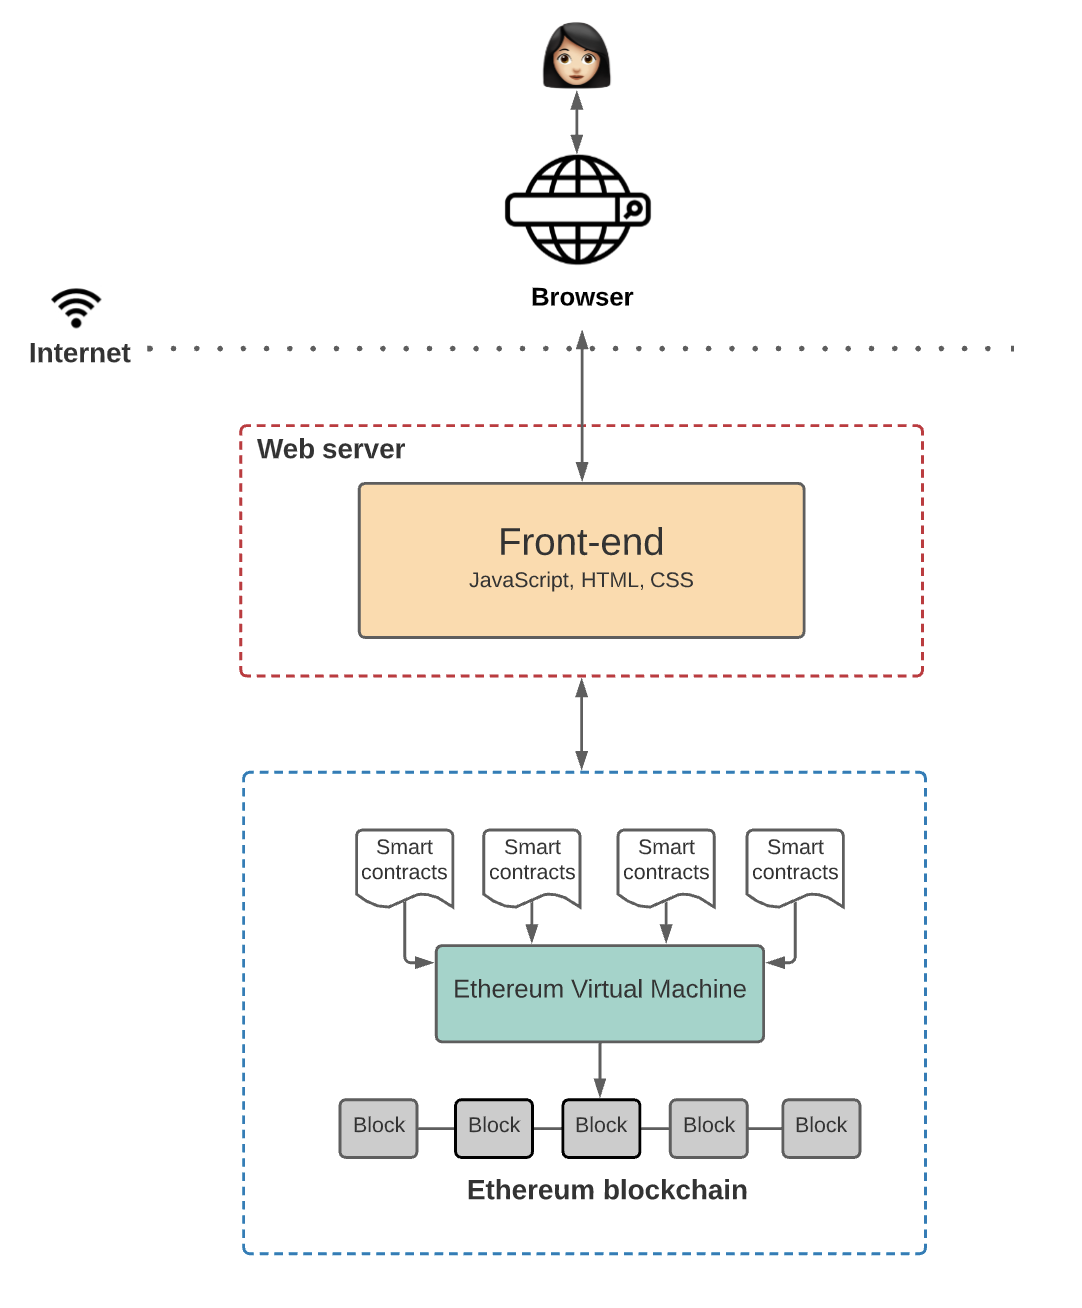
\includegraphics[width=0.65\textwidth]{Immagini/web_30.png}
\end{figure}
